\chapter{Systemmodels}
\label{ch:sysmodels}

\section{System architecture}
The specified criteria demand for a minimalist user interface and little to no bidirectional data flow within the application. Therefore the applied architecture will be a modified version of the classic pipeline architecture.

\subsection{Basic Pipeline}
The traditional pipeline architecture refers to a process being split up into several sequential step, ideally with data buffers in between those, which can will be able to independently and possibly asynchronously perform a specific work on their data input, which will then be provided as output for the subsequent step. This works especially well in scenario were only an unidirectional data flow is required.

\subsection{The extended pipeline}
In this project, the basic pipeline is an insufficient model, as the initial input data will have to be gathered at several, mostly independent places. The \gls{browser} module (see \specref{FS220} will only capture \gls{browser} \glspl{event}, the window management \gls{module} (see \specref{FS180}) cannot also provide the keyboard input etc. In order to solidify all the collected \glspl{event}, the extended pipeline allows for a single processing step to accept input from multiple sources by utilizing the transforming modules as mentioned in \specref{FS170}. The result is a tree-structure where the \gls{event}-data strictly flows from the leafs towards the root, the root being the application core (see \specref{FS140}).

\section{Object models}

\section{Dynamic models}
Following figure shows exemplarily how the application could deal with a user clicking on an element in his webbrowser. The actual flow might differ based on available modules and rule configuration.
\begin{figure}[h!]
  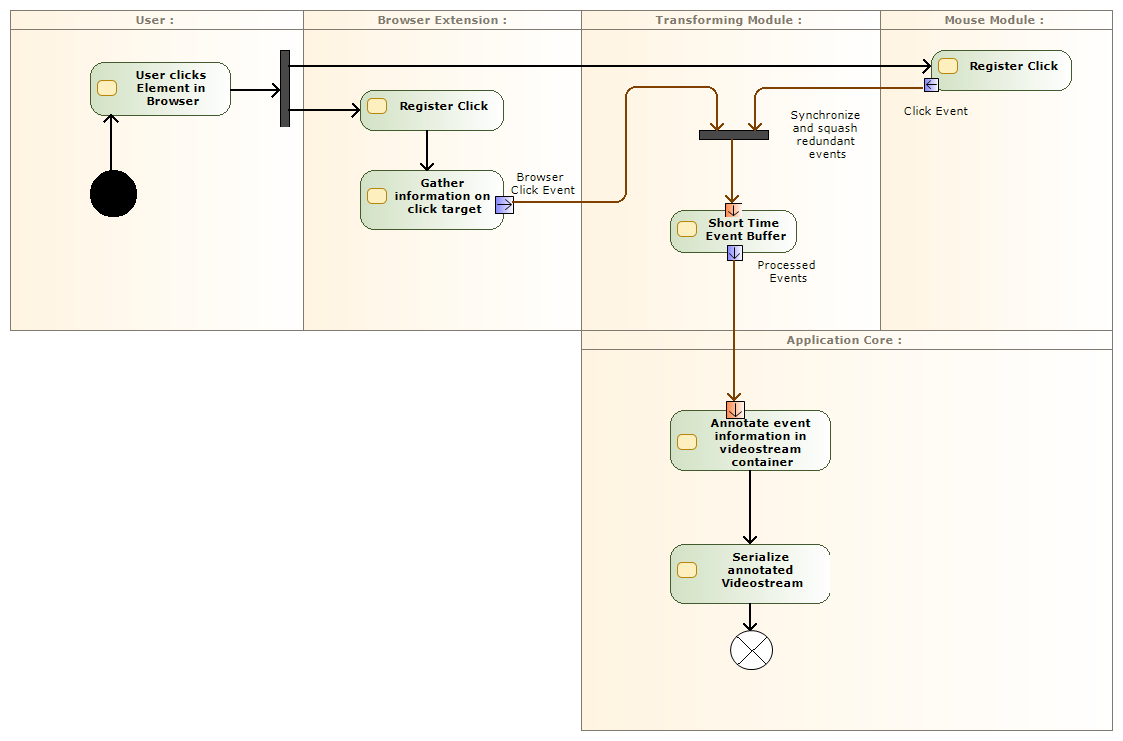
\includegraphics[width=1.00\textwidth]{resources/clickactivity.png}
  \centering
  \caption{User-Click sample activity chart}
  \label{fig:clickactivity}
\end{figure}
\section{User Interface}
